\section{Metodología}\label{Metodología}

\subsection{Enfoque de la investigación}

En esta investigación se empleará un enfoque cuantitativo, con el objetivo de analizar de manera objetiva y cuantificable la relación entre la resolución de la guía de programación y el éxito académico en el curso de Introducción a la Programación de la Universidad Andrés Bello.

\subsection{Diseño de investigación}

Se empleará la metodología KDD (Knowledge Discovery in Databases) para llevar a cabo el análisis de los datos. El proceso de KDD consta de varias etapas fundamentales que nos permitirán obtener conocimientos relevantes a partir de los datos recopilados.

\begin{figure}[H]
  \centering
  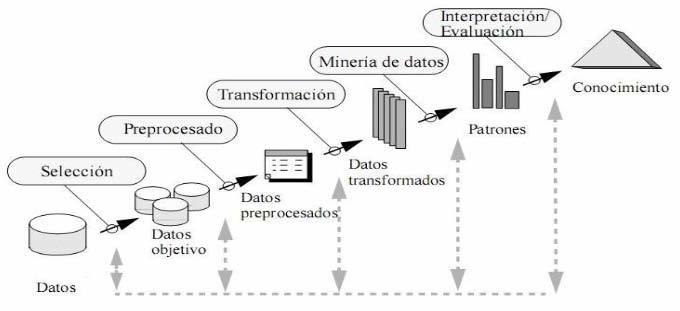
\includegraphics[width=0.5\textwidth]{img/KDD.png}
  \caption{Flujo gráfico KDD}
  \label{fig:flujo_kdd}
\end{figure}

A continuación, se describen las etapas del proceso KDD y cómo se adaptan a esta investigación:

\begin{enumerate}
  \item \textbf{Selección:} En esta etapa, se determinan y seleccionan los conjuntos de datos relevantes para la investigación. En el contexto de esta tesis, se seleccionarán los datos relacionados con el rendimiento académico y la resolución de guías de programación.

  \item \textbf{Preprocesamiento:} Se limpian y transforman los datos para eliminar cualquier inconsistencia o error. Para esta tesis, se realizará una limpieza de los datos para garantizar que no haya valores faltantes o atípicos que puedan afectar el análisis.

  \item \textbf{Transformación:} Los datos se transforman en un formato adecuado para el análisis. En el caso de esta investigación, se podrían realizar transformaciones como la normalización o la codificación de variables categóricas.

  \item \textbf{Minería de datos:} Se aplican técnicas de análisis para extraer patrones y conocimientos de los datos. En esta tesis, se emplearán las técnicas SHAP y DoWhy. SHAP se utilizará para analizar la importancia de las características y su relación con el rendimiento académico, mientras que DoWhy se empleará para la inferencia causal, permitiendo entender las relaciones causales subyacentes en los datos.

  \item \textbf{Interpretación/Evaluación:} Los resultados obtenidos en la etapa anterior se interpretan y evalúan en función de su relevancia y utilidad. En el contexto de esta investigación, se discutirán los hallazgos y se evaluará su significado en relación con la pregunta de investigación planteada.
\end{enumerate}

Estas etapas garantizan un enfoque sistemático y riguroso para el análisis de datos, asegurando que los resultados obtenidos sean relevantes y confiables para la investigación.


\subsection{Análisis de la base de datos}

Se utiliza un conjunto de datos que registra a los estudiantes que tomaron el curso de Introducción a la Programación en la Universidad Andrés Bello durante el año 2021. Estos datos incluyen información sobre el rendimiento de los estudiantes en la resolución de la guía de apoyo para la primera evaluación.

\subsubsection{Definición de la variable objetivo}

Dado que el objetivo de esta investigación es determinar si la resolución de la guía tiene algún impacto en la aprobación de la prueba de evaluación del curso, se propone utilizar la variable \say{sol1} como variable objetivo. Dado que esta variable es de tipo cuantitativa, se sugiere generar una nueva columna llamada aprobado, la cual será de tipo binaria. En esta columna, se representará con el valor 1 a las notas superiores a 4.0 hasta la nota máxima de 7.0, mientras que se asignará el valor 0 a aquellas notas inferiores a las indicadas, representando la condición de reprobado.

\subsection{Comparador de Algoritmos}

Para determinar el mejor modelo de clasificación y regresión, se utilizará un comparador de algoritmos. Este comparador evaluará el rendimiento de varios modelos, incluyendo DecisionTreeClassifier, LogisticRegression, RandomForestClassifier, XGBClassifier, LinearRegression, DecisionTreeRegressor y KNeighborsRegressor, utilizando métricas específicas para cada tipo de modelo.

\begin{figure}[H]
  \centering
  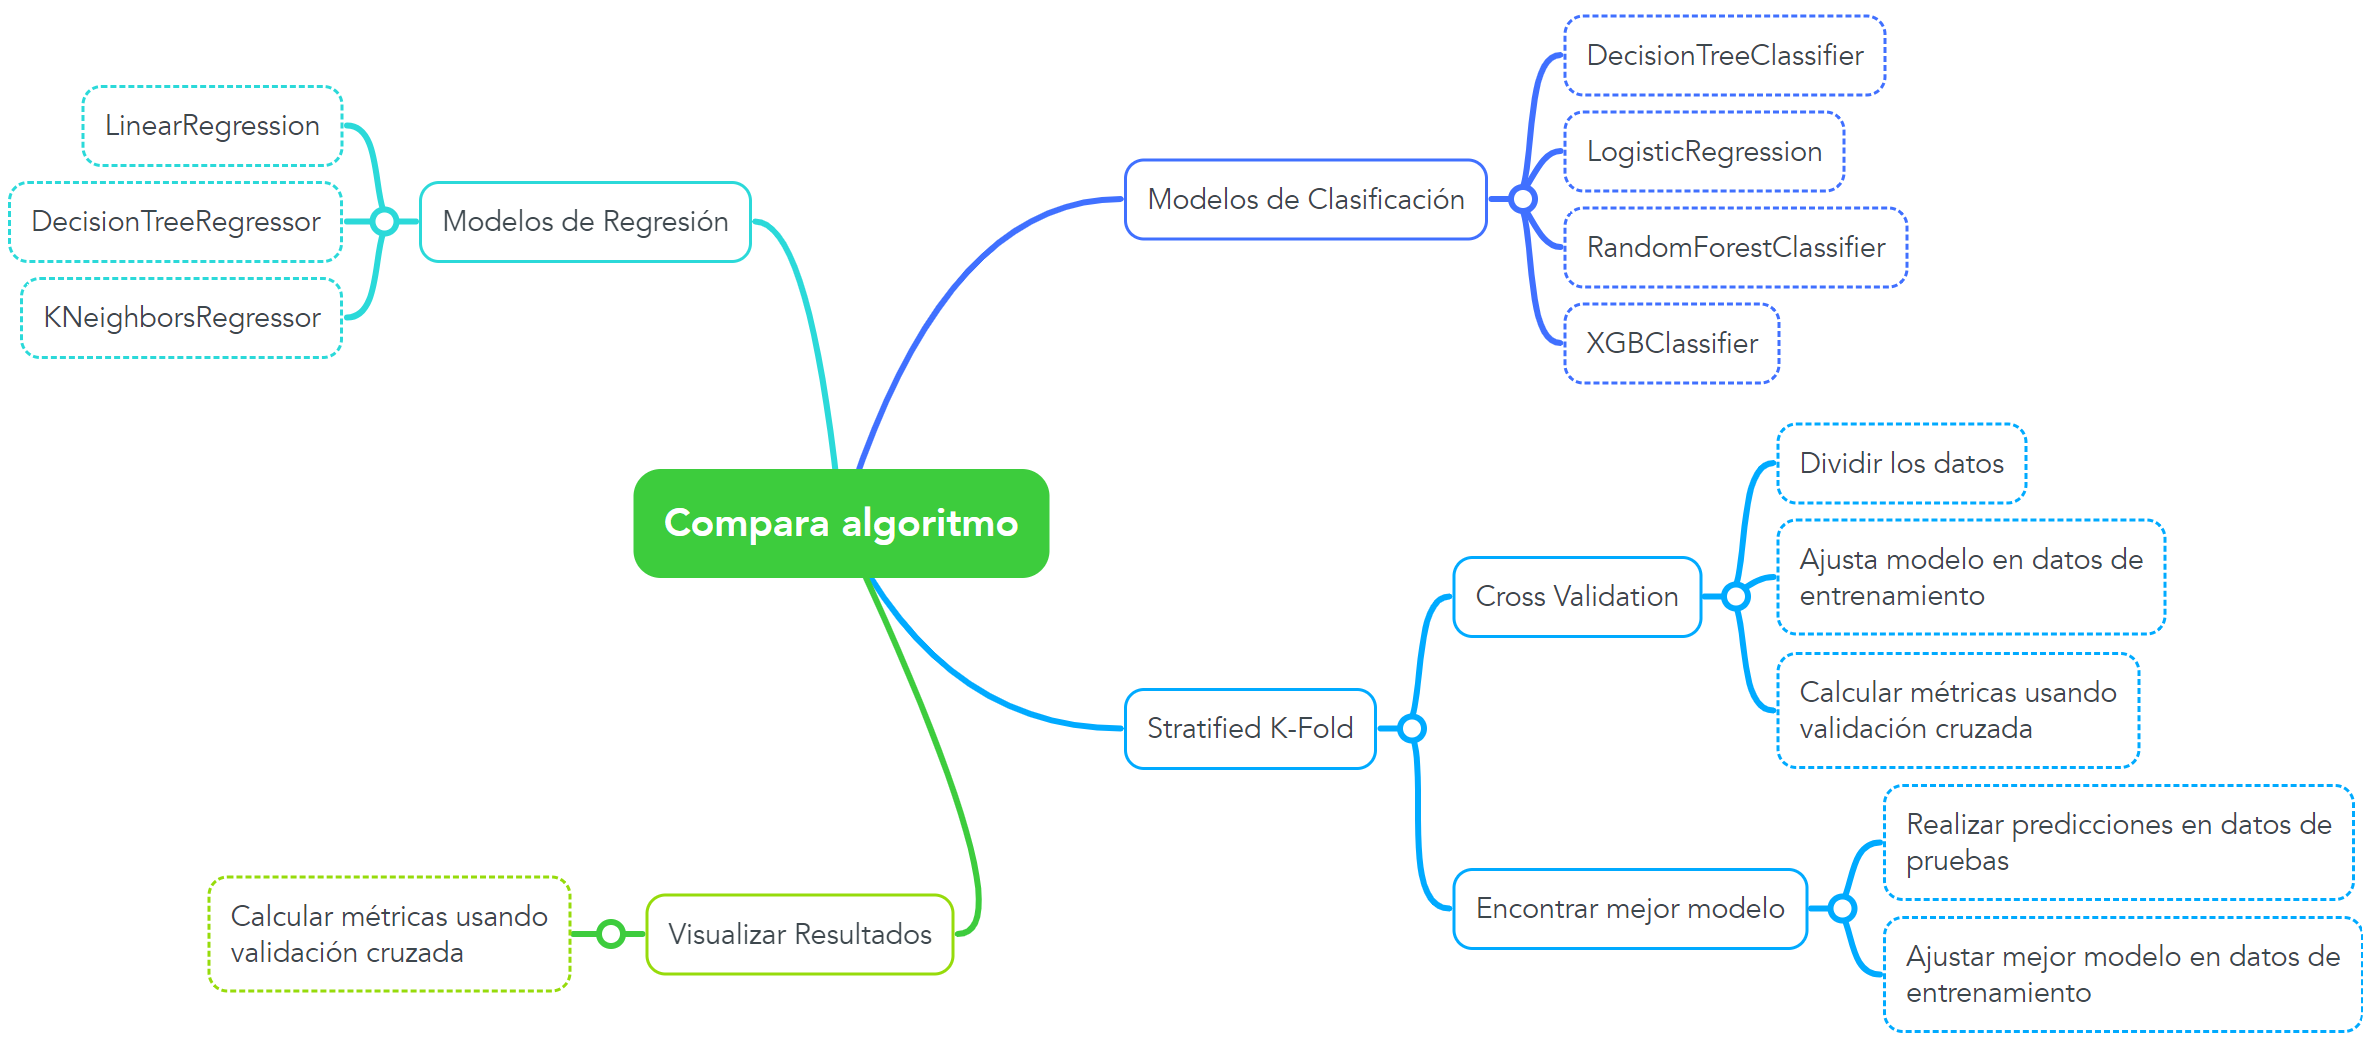
\includegraphics[width=1\textwidth]{img/compara_algoritmos/comparaAlgoritmoCompletoMindMap.png}
  \caption{Mind Map de comparador de algoritmos}
  \label{fig:mindMap_comparaAlgoritmos}
\end{figure}

\subsubsection{K-Fold Cross-Validation y Stratified K-Fold Cross-Validation}

La validación cruzada de K particiones, o K-Fold CV, es una técnica de evaluación de modelos que divide el conjunto de datos en K particiones (subconjuntos) de igual tamaño. En cada iteración del proceso de validación cruzada, se utiliza una de las particiones como conjunto de prueba y las K-1 particiones restantes como conjunto de entrenamiento. Esto se repite K veces, utilizando una partición diferente como conjunto de prueba en cada iteración. Al final, se calcula el promedio de las métricas de evaluación obtenidas en cada iteración para tener una medida general del rendimiento del modelo.

La validación cruzada estratificada de K particiones, o Stratified K-Fold CV, es una variante de K-Fold CV que tiene en cuenta la distribución de las clases en los datos al realizar la partición. En lugar de realizar la partición de forma aleatoria, Stratified K-Fold CV garantiza que la proporción de clases en cada partición sea lo más similar posible a la proporción de clases en el conjunto de datos original.

\begin{figure}[H]
  \centering
  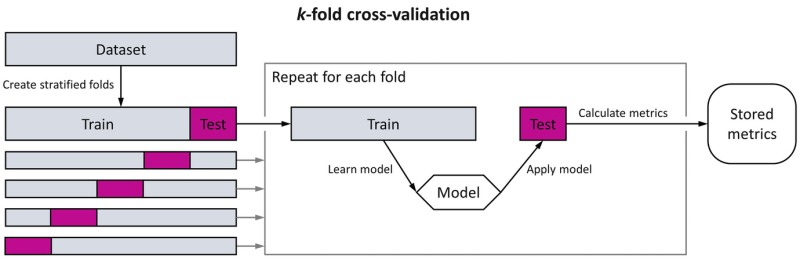
\includegraphics[width=0.5\textwidth]{img/analisis de metodologia/463627_1_En_8_Fig8_HTML.jpg}
  \caption{Flujo gráfico Tecnicas combinadas Stratified K-Fold CV}
  \label{fig:flujo_kfoldcvstratfield}
\end{figure}

\subsection{Comparación de Métricas entre Modelos de Clasificación}

Se utilizarán diversas métricas, incluyendo precisión, exhaustividad, F1-score, entre otras, para proporcionar una visión completa del rendimiento de cada modelo de clasificación. Las fórmulas para estas métricas se presentarán a continuación.

\subsubsection{Accuracy}
El accuracy, o precisión, es una métrica que mide la proporción de instancias clasificadas correctamente sobre el total de instancias en los datos de prueba. Es una medida general del rendimiento del modelo en la clasificación. El valor de accuracy se calcula utilizando la siguiente fórmula:

\begin{equation}
  \text{Accuracy} = \frac{\text{Verdaderos Positivos + Verdaderos Negativos}}{\text{Total de instancias}}
\end{equation}

Un valor de accuracy alto indica un buen rendimiento general del modelo en la clasificación.

\subsubsection{Precision}
La precisión es una métrica que mide la proporción de instancias clasificadas como positivas que son realmente positivas. Es la capacidad del modelo para evitar hacer falsas afirmaciones de que una instancia pertenece a la clase positiva cuando no lo hace. La precisión se calcula utilizando la siguiente fórmula:

\begin{equation}
  \text{Precision} = \frac{\text{Verdaderos Positivos}}{\text{Verdaderos Positivos + Falsos Positivos}}
\end{equation}

Una precisión alta indica que el modelo tiene una baja tasa de falsos positivos.

\subsubsection{Recall}
El recall, también conocido como sensibilidad o tasa de verdaderos positivos, mide la proporción de instancias positivas que son correctamente identificadas por el modelo. Es la capacidad del modelo para detectar y clasificar correctamente las instancias positivas. El recall se calcula utilizando la siguiente fórmula:

\begin{equation}
  \text{Recall} = \frac{\text{Verdaderos Positivos}}{\text{Verdaderos Positivos + Falsos Negativos}}
\end{equation}

Un recall alto indica que el modelo tiene una baja tasa de falsos negativos.

\subsubsection{F1 Score}
El F1 score es una métrica que combina la precisión y el recall en una sola medida. Es la media armónica de la precisión y el recall, y proporciona una evaluación equilibrada del rendimiento del modelo. El F1 score se calcula utilizando la siguiente fórmula:

\begin{equation}
  \text{F1 Score} = \frac{2 \cdot (Precision \cdot Recall)}{Precision + Recall}
\end{equation}

El F1 score es especialmente útil cuando hay un desequilibrio entre las clases o cuando se desea tener un equilibrio entre la precisión y el recall.

\subsection{Medidas de Rendimiento de Modelos de Regresión}

Se utilizarán métricas como el error cuadrático medio y el coeficiente de determinación para evaluar el rendimiento de los modelos de regresión. Las fórmulas para estas métricas se presentarán a continuación.

\subsubsection{MSE (Mean Squared Error) - Error Cuadrático Medio}
El MSE es la media de los errores al cuadrado entre las predicciones y los valores reales. El MSE proporciona una medida de la calidad general del modelo, donde valores más bajos indican que las predicciones se ajustan mejor a los datos reales.

\subsubsection{MAE (Mean Absolute Error) - Error Absoluto Medio}
El MAE es la media de los errores absolutos entre las predicciones y los valores reales. El MAE representa la magnitud promedio de los errores de predicción y se utiliza para evaluar la precisión del modelo. Valores más bajos indican una mejor precisión.

\subsubsection{R2 (Coeficiente de determinación)}
El R2 es una medida de qué tan bien se ajustan las predicciones del modelo a los datos reales. R2 varía entre 0 y 1, donde 1 indica un ajuste perfecto del modelo a los datos. Un valor más cercano a 1 indica un mejor ajuste del modelo.

\subsection{Aplicación de XAI y SHAP para el Mejor Modelo}

Las técnicas de XAI (Explainable Artificial Intelligence) y SHAP (Shapley Additive exPlanations) se aplicarán al modelo que haya demostrado el mejor rendimiento en el comparador de algoritmos. Estas técnicas proporcionarán insights sobre qué características son las más influyentes en las predicciones del modelo y cómo estas características afectan las decisiones del modelo.

\textbf{XAI (Explainable Artificial Intelligence):} XAI se refiere a métodos y técnicas en el dominio de la inteligencia artificial (IA) que son interpretables y comprensibles por seres humanos. La idea es que un ser humano pueda entender el proceso completo de toma de decisiones de un modelo de IA. Esto es esencial para construir la confianza y permitir a los humanos entender, aprobar o rechazar las decisiones tomadas por los algoritmos de IA.

\textbf{SHAP (Shapley Additive exPlanations):} SHAP es una técnica que se basa en la teoría de juegos para explicar la salida de cualquier modelo de aprendizaje automático. Proporciona una medida de la importancia de cada característica en la predicción para una observación individual en el contexto de un modelo. Los valores SHAP interpretan el impacto de tener una característica en particular en comparación con la expectativa del modelo sobre todas las posibles combinaciones de características.

\begin{figure}[H]
  \centering
  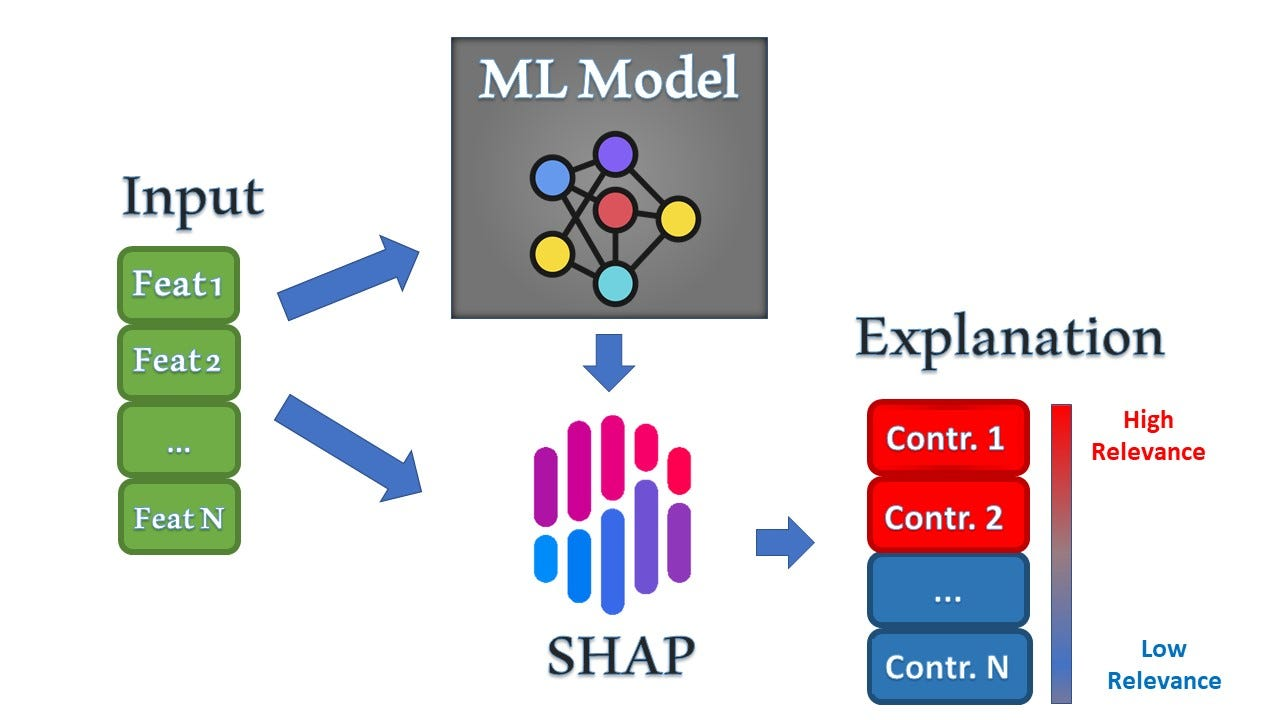
\includegraphics[width=0.5\textwidth]{img/xai_shap.jpg}
  \caption{Interpretación de resultados con XAI y SHAP}
  \label{fig:xai_shap}
\end{figure}


\subsection{Análisis de Causalidad con DoWhy}

El análisis de causalidad va más allá de la simple correlación, buscando identificar relaciones directas de causa y efecto entre variables. En el ámbito de la minería de datos y el aprendizaje automático, esta distinción es crucial para tomar decisiones informadas basadas en los resultados de un modelo.

\textbf{DoWhy:} DoWhy es una biblioteca de Python que se centra en la inferencia causal. Su objetivo es no solo proporcionar herramientas para realizar análisis causal, sino también guiar al usuario a través del proceso lógico y empírico de inferencia causal. Se basa en la idea de que la inferencia causal requiere dos pasos: primero, modelar el proceso generativo de los datos y, segundo, utilizar técnicas estadísticas para identificar efectos causales a partir de datos observados.

En el contexto de esta investigación, DoWhy se utilizará para analizar la relación causal entre la resolución de la guía de programación y el éxito académico. Aunque puede haber una correlación observada entre estos dos factores, es esencial determinar si la resolución de la guía tiene un efecto directo en el rendimiento académico o si hay otras variables no observadas que puedan estar influyendo en ambos.

Para llevar a cabo este análisis, se identificarán variables de confusión potenciales que puedan afectar tanto la resolución de la guía como el rendimiento académico. Una vez identificadas, se aplicarán técnicas como el matching de propensión para controlar estos factores y obtener estimaciones causales más precisas. El matching de propensión es una técnica que busca emparejar individuos con características similares pero con diferentes tratamientos (en este caso, resolver o no la guía) para comparar sus resultados y determinar el efecto causal del tratamiento.

\begin{figure}[H]
  \centering
  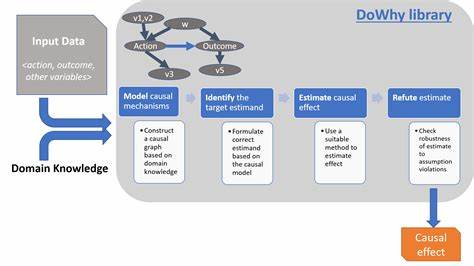
\includegraphics[width=0.5\textwidth]{img/dowhy.jpg}
  \caption{Flujo DoWhy librería Python}
  \label{fig:dowhy_lib}
\end{figure}

En resumen, el análisis de causalidad con DoWhy proporcionará insights valiosos sobre la verdadera relación entre la resolución de guías de programación y el éxito académico, permitiendo a los educadores y responsables de la toma de decisiones actuar con base en evidencia causal y no solo en correlaciones observadas.


\subsection{Conclusiones}

Con la aplicación de la metodología descrita, se espera obtener una comprensión profunda de la relación entre la resolución de la guía de programación y el éxito académico en el curso de Introducción a la Programación en la Universidad Andrés Bello. Las técnicas y herramientas seleccionadas permitirán identificar patrones, relaciones y factores influyentes que pueden ser utilizados para mejorar los procesos de enseñanza y aprendizaje.